 
\documentclass[12pt]{article}

\usepackage[margin=0.8 in]{geometry}
\usepackage{amsmath}
\usepackage{amssymb}
\usepackage{mathtools}
\usepackage{enumerate}
\usepackage{verbatim}
\usepackage{amsthm}
\usepackage{hyperref}

\title{Worksheet 3}
%\content{}



\let \proj \undefined
\newcommand{\p}{\partial}
\newcommand{\R}{ \mathbb{R}}

\DeclareMathOperator{\proj}{proj}
\newcommand{\sS}{\mathscr{S}}
\DeclareMathOperator{\comp}{comp}
\newcommand{\A}{\mathcal{A}}
\newcommand{\D}{\mathcal{D}}
\newcommand{\e}{\epsilon}
\newcommand{\et}{\tilde{\e}}
\newcommand{\vr}{\vec{r}{}}
\newcommand{\vF}{\vec{F}}
\newcommand{\triple}{\iiint_E f(x,y,z)dV}
\renewcommand{\lg}{\langle}
\newcommand{\rg}{\rangle}
\newcommand{\Q}{\frac{\p Q}{\p x}}
\renewcommand{\P}{\frac{\p P}{\p y}}
\let\implies\Rightarrow
\newcommand{\n}{\nabla}
\newcommand{\Fline}{\vF\cdot d\vr}
\newcommand{\vi}{\vec{i}}
\newcommand{\vj}{\vec{j}}
\newcommand{\vk}{\vec{k}}
\DeclareMathOperator{\curl}{curl}

\newcommand{\vn}{\vec{n}}
\newcommand{\vS}{\vec{S}}
\newcommand{\flux}{\iint_S \vF\cdot d\vS}


\newcommand{\rcross}{\vr_u\times\vr_v}

\let \div\undefined
\DeclareMathOperator{\div}{div}

\newenvironment{solution}
  {\begin{proof}[Solution]}
  {\end{proof}

  }
\newtheorem{example}{Example}
\newtheorem{exercise}{Exercise}
\newtheorem{theorem}{Theorem}
\newtheorem{defn}{Definition}


\begin{document}
%\section*{Worksheet 3}
\maketitle
\begin{enumerate}
\item Decide which of the three plots below corresponds to the parametrization $$\vr(u,v)=\lg \left (2+\cos(v)\right )\cos(u),\left  (2+\cos(v)\right  )\sin(u),\sin(v)\rg, \text{ for }(u,v)\in[0,2\pi]\times [0,2\pi]$$
\begin{figure}[h]
\minipage{0.32\textwidth}
  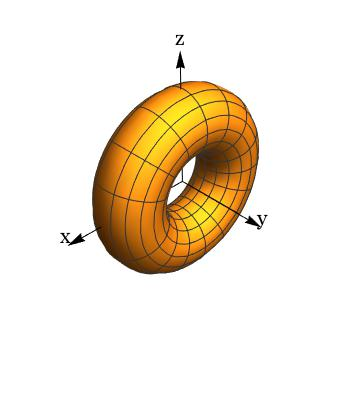
\includegraphics[width=\linewidth]{torus2.jpeg}
  \caption{Plot 1}
\endminipage\hfill
\minipage{0.32\textwidth}
  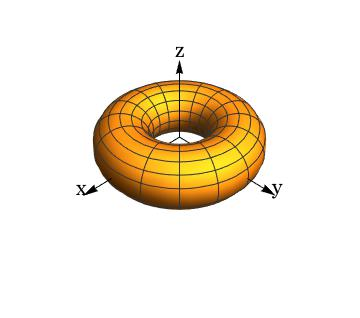
\includegraphics[width=\linewidth]{torus1.jpeg}
  \caption{Plot 2}
\endminipage\hfill
\minipage{0.32\textwidth}%
  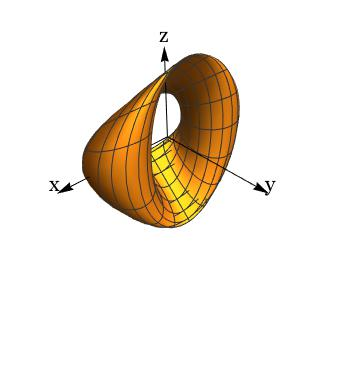
\includegraphics[width=\linewidth]{sth.jpeg}
  \caption{Plot 3}
\endminipage
\end{figure}

\item Prove the first step towards showing Green's First Identity: Show that for any twice differentiable functions $u(x,y,z)$ and $v(x,y,z)$ we have \begin{equation}
\label{eq1} \div(u\n v)=\n u\cdot\n v+u\Delta v
\end{equation}

\begin{comment}
\item Prove Green's First Identity (or Green's Symmetric Formula): \\

Let $E$ be a domain in $\R^3$ and $\p E$ its positively oriented boundary with unit normal $\vec{n}$. Then, if $u$, $v$ are twice differentiable scalar valued functions on $\R^3$, we have \begin{equation}\label{green}\iint_{\p E} vD_{\vn}u-u D_{\vn}vdS=\iiint_Ev\Delta u-u\Delta vdV.
\end{equation} Here are the steps:

\begin{enumerate}
\item Show that for any twice differentiable functions $u(x,y,z)$ and $v(x,y,z)$ we have \begin{equation}
\label{eq1} \div(u\n v)=\n u\cdot\n v+u\Delta v
\end{equation}
and
\begin{equation}
\div(v\n u)=\n v\cdot\n u+v\Delta u\label{eq2}.
\end{equation}
\item Subtract \eqref{eq1} from \eqref{eq2}
\item Apply the Divergence Theorem on the left hand side of the resulting equation.
\item Use the formula $D_{\vec{u}}f=\nabla f\cdot \vec{u}$ (where $\vec{u}$ is a unit vector) for directional derivatives to rewrite the resulting equation into \eqref{green}.
\end{enumerate}
\end{comment}


%\vspace{2 in}
\vfill


\item Compute the line integral $\int_c \Fline$, where $\vF=\lg -y,x,2\rg$ and $c$ is the path that consists of the following line segments, as in Figure \ref{fig2}:
\begin{itemize}
\item A line segment from $(0,0,1)$ to $(-1,1,0)$.
\item A line segment from $(-1,1,0)$ to $(1,1,0)$.
\item A line segment from $(1,1,0)$  back to $(0,0,1)$.
\end{itemize}

\vfill
\newpage

\item Let $S$ be the surface that consists of the part of the cylinder $x^2+y^2=1$ lying between the planes $z=0$ and $z=-1$, together with the part of the sphere $$x^2+y^2+(z+1+\sqrt{3})^2=4$$ that lies below the plane $z=-1$, and let $S$ have orientation pointing away from the origin, as in picture \ref{fig1}. 

\begin{enumerate}
\item Compute $\int_S \vF\cdot d\vec{S}$, where $\vF(x,y,z)=\langle y+x, x+z,-z+y^2\rangle$.\\
 Hint: Modify the surface accordingly so you can use divergence theorem.

\item *Find the surface area of $S$.
\end{enumerate}



 \begin{figure}[h]
 \begin{center}


 \end{center}
 \end{figure}
 
\begin{figure}
\centering
\parbox{5cm}{
 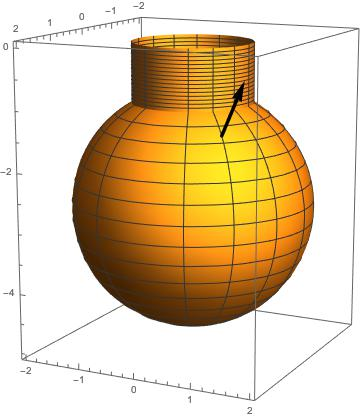
\includegraphics[width=5cm]{grenade.jpeg}
 \caption{Problem 4}
 \label{fig1}}
\qquad
\begin{minipage}{5cm}
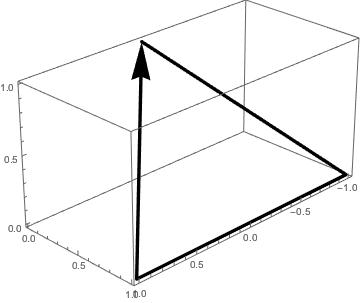
\includegraphics[width=5cm]{path.jpeg}
\caption{Problem 3}
\label{fig2}
\end{minipage}
\end{figure} 
 




\end{enumerate}







\end{document}
